\documentclass{article}

\usepackage{geometry}
\usepackage{a4}
\usepackage{amsmath}
\usepackage{graphicx}
\usepackage{svg}

\geometry{left=2cm, right=2cm, top=2cm, bottom=2cm}

\title{Simulation of Wireless Communication}
\author{Logan Brown 2641407B}

\begin{document}

\maketitle
\section{Overview}
\subsection{Simulation}
The main aim of this simulation was to be able to visualise the demodulation of a GIF happening in real time, with the option to dynamically alter the signal-to-noise ratio (SNR) of the system, using Additive Gaussian White Noise (AGWN). The two key constraints imposed by this were the memory usage of the program, and the speed of processing the simulation.

With a simulation not done in real time, there is no real limit imposed by the speed of processing the simulation, other than the user's patience. However, when simulating in real time, the simulation has to run fast enough that the demodulation can happen at least as fast as real time.

As well as this, a GIF contains a large amount of data, which quickly eats up memory when simulating its transmission. If the sampling rate is 100 times the bit transmission rate, and 64-bit floating point numbers are used, then simulating the transmission of a 400x400 pixel GIF containing 50 frames with a colour depth of 3 bytes would require 3 gigabytes of memory.

\begin{equation}
    \begin{aligned}
             & w \times h \times d \times n_{\text{frames}} \times 8 \times 100 \times 4                  \\
        = \: & 400 \times 400 \times 3 \times 50 \times 8 \times 100 \times 4 \approx 3 \text{ GB} \notag
    \end{aligned}
\end{equation}

To make this simulation work, a few tradeoffs had to be made: the resolution of the GIF was set to 40x40 pixels; the modulation of the signal, as well as any filtering on the receiving end, would be done ahead of time; and lower-precision (32-bit) floating point numbers would be used. To avoid dealing with frequency scaling issues, the samples were split into 1 second bins before performing the Fast Fourier Transform (FFT) required for frequency filtering, which also meant that the memory usage was much lower, since it did not require copying the whole sample space at once. In addition to this, AGWN has frequency components across the spectrum, and as such it does not matter whether it is added before or after filtering. I chose to write the simulation code in Java, as it gives more control over memory usage and lower level operations, as well as executing significantly faster. Since this is a relatively complex project, it was also helpful to have a language which scales much better than either Python or Mathematica.

The system may be visualised using the diagram below. 

\noindent
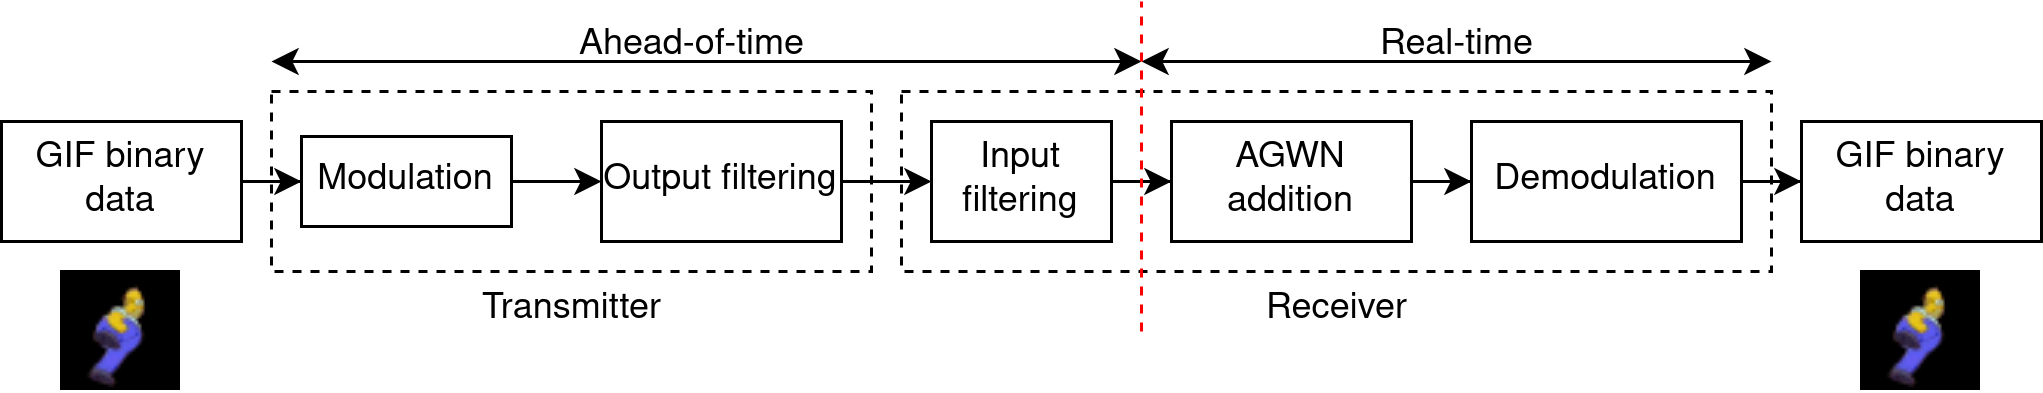
\includegraphics[width=\textwidth]{figures/system-diagram.png}

\subsection{Modulation}
Two modulation formats were implemented: Amplitude Shift Keying (ASK), and Quadrature Amplitude Modulation (QAM). I also intended to implement Frequency Shift Keying, but this was not possible due to the time constraints imposed by the rest of the project. Unfortunately, I was not able to get either format quite working properly, as they seem to work fine for the first frames of the GIF, but then degrade for the later ones. However, as they behave as expected for the first frames of the GIF (transmitting well over the 2048 bit requirement in that time), useful results were still obtained.

\section{Results}
The three most important metrics of a good modulation scheme are the bit error rate (BER), the spectral efficiency, and the transmission rate. Any modulation scheme will make a tradeoff between these three, but some do better in this regard than others. For each of the following tests, the carrier frequency was set to 10 kHz, the modulation frequency was set to 1 kHz, and the carrier amplitude was set to 100 units. For ASK, the depth used was 0.5 (as a fraction of the carrier amplitude), and for QAM the order was 16.   

\subsection{Bit error rate (BER)}
From five transmissions of five frames:
\begin{center}
    \begin{tabular}{|c|c|c|}
        \hline
                 & \multicolumn{2}{c|}{Modulation Scheme}         \\ \hline
                 & ASK                                    & QAM   \\ \hline
        SNR (dB) & \multicolumn{2}{c|}{BER (mean)}                \\ \hline
        24       & 0                                      & 0.07  \\
        18       & 0.003                                  & 0.07  \\
        6        & 0.823                                  & 0.114 \\ \hline
    \end{tabular}
\end{center}

QAM appears to have some baseline bit error as opposed to ASK (which has 0 bit errors at high SNR), but is less susceptible to noise, with a much lower BER at 6 dB than ASK. I believe the baseline BER of QAM may be due to either an error in my implementation of the scheme, or due to the inherent innaccuracies of the simulation, either in the lower-precision floating point numbers, or the FFT implementation.

\subsection{Spectral efficiency}
To test the spectral efficiency of the two formats, the BER of each was measured for a number of different bandwidths, each a percentage of the carrier frequency. 


\end{document}